\documentclass[]{beamer}
\usepackage[MeX]{polski}
\usepackage[cp1250]{inputenc}
%\usepackage{polski}
%\usepackage[utf8]{inputenc}
\beamersetaveragebackground{blue!10}
\usetheme{Warsaw}
\usecolortheme[rgb={0.1,0.5,0.7}]{structure}
\usepackage{beamerthemesplit}
\usepackage{multirow}
\usepackage{multicol}
\usepackage{array}
\usepackage{graphicx}
\usepackage{enumerate}
\usepackage{amsmath} %pakiet matematyczny
\usepackage{amssymb} %pakiet dodatkowych symboli

\title{Prezentacja na temat \TeX a}
\date{}

\begin{document}

\frame
{
\frametitle{Blocki w \TeX u}
\begin{block}
{Przyk�adowy blok w \TeX u}
Tu wpisujemy tre��
\end{block}
\begin{exampleblock}
{A to jest blok do przyk�ad�w}
Na przyk�ad
\end{exampleblock}
\begin{alertblock}
{Uwaga!}
U�ywamy gdy chcemy podkre�li� co� wa�nego
\end{alertblock}
}
\frame
{
 \frametitle{Podpunkty i widoczno��}
Zagadnienia z \TeX a, kt�re omawiali�my na �wiczeniach
 \begin{itemize}
  \item<1-4> sk�adanie tekstu w \TeX u
	\item<2-4> wzory matematyczne i �rodowisko algoritmic
	\item<3-4> tabele, rysunki
	\item<4-4> pakiet beamer - do tworzenia prezentacji
 \end{itemize}
 \begin{enumerate}
  \item sk�adanie tekstu w \TeX u \pause
	\item wzory matematyczne i �rodowisko algoritmic \pause
	\item tabele, rysunki \pause
	\item pakiet beamer - do tworzenia prezentacji
 \end{enumerate}
}
\frame
{
 \frametitle{Wz�r Matematyczny}
 \begin{displaymath}
  a^2+b+c+5=0
 \end{displaymath}
}
\frame
{
 \frametitle{Tabele}
\begin{table}
	\centering
		\begin{tabular}{|c|c|c|c|c|} \cline{1-5}
			  & \multicolumn{4}{c|}{ 2 3 4 5} \\
		 \hline
		 \pause

       \multirow{3}{*}{asd} & 2 & 3 & 4 & 5 \\ \cline{2-5}
        & 2 & 3 & 4 & 5 \\ \cline{2-5}
		    & 5 & 4 & 3 & 2 \\
		\hline
		\end{tabular}
\end{table}
}
\frame
{
 \frametitle{Obrazek}
  \begin{figure}[here]
	\begin{center}
	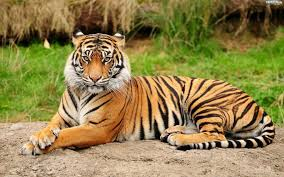
\includegraphics[scale= 0.4]{tygrys.jpg}
	\end{center}
	\end{figure}
}
\frame
{
 \begin{columns}
 \frametitle{Column}
  \column{0.3 \textwidth}
   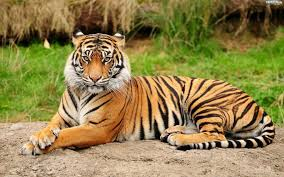
\includegraphics[scale= 0.3]{tygrys.jpg}
  \column{0.4 \textwidth}
   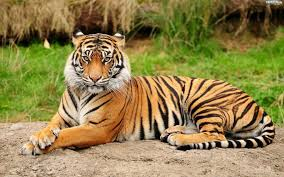
\includegraphics[scale= 0.4]{tygrys.jpg}
 \end{columns}
}

\end{document}